% !TEX root = ../main.tex

% = = = = = = = = = = = = = = = = = = = = = = = = = = = = = = = = = = = = = = = = = =

\section{Introductory Remarks}



\section{Classification}

\subsection{Retail Changes}
This is not a standardized pattern. The development team must consider the ways to upgrade the contracts before deploying the smart contract. Known patterns are different on the level of intervention to change the logic that they need to change in the future. The amount of changes are limited and system design can not be changed after deployment and just some system variables can be changed. We will describe three famous patterns here:

\paragraph{Parameter Configuration}. The easiest way to upgrade the logic of the smart contract is to have some critical parameter that can change the whole logic of the system. For instance, in economy we have different variables which have effect in the interest rates. By changing those variables the governors will response to changes needed for the system. 
In this model we have a setter function to change the upgradable parameters if the system needs upgrades. The best example for this type of upgradeability is MakeDao project. In Maker there are some variables like Dai Saving Rate (DSR) or Stability fee that can be changed through governance vote. The logic behind the smart contract and the tokenomic of the Dapp completely depends on these variables.

\paragraph{Strategy pattern}. The strategy pattern is an easy way for changing part of the code in a contract responsible for a specific feature. Instead of implementing a function in your contract to take care of a specific task, you call into a separate contract to take care of that – and by switching implementations of that contract, you can switch between different strategies.
An example for this pattern is Compound project and how they used strategy pattern for their interest rate model. There is a interest rate model contract in Compound that can be changed during the time. 

\paragraph{Pluggable Modules}. In this pattern we have a core contract that have some immutable features and then new contracts generated by the main contract and each have some or all features of the main contract. This pattern is mostly used in wallets and DeFi services like DeFi saver and InstaDapp. Users can decide to add new features into their wallet. 

%TODO: Ask shayan about DeFi save and how do they upgrade their contracts.
\subsection{Wholesale Changes}
In contrast to previous session, sometime we need to change the whole or a big part of the logic of our smart contract. This update could be a response to an incident happen to the smart contract or a planed upgrade of the system. Before deployment, the core developer team should have a plan for the upgrade events. We categorized these types into two main classes:

\subsubsection{Contract Migration}
%who will push the old data? user to provide its own data to the new version?
In the migration plan we should write a completely new contract with our desired new logic. In migration method our new version contract doesn't have any communication with the previous versions. The challenges we face in migration method are:
\begin{enumerate}
    \item Grab the needed data (from previous contract or new data): 
    It depends on the data type. It is easy for simple data structures (\eg uint, address, or even arrays) to collect the data just by reading storage slots from the 0 slot. we should take care of complex structures (\eg mapping) in the latest versions of our contract by adding event updates whenever a data added to a mapping variable. In case of an upgrade we can use Logs to find storage slot (using key hash) and collect the data.
    Sometime we need to push new data into our upgraded smart contract. For example in airdrops we need new coin to be added to some specific addresses. 
    \item Push the data into the new contract: 
    Using Constructor, we can use batch transfer function with arrays of addresses and amounts as inputs. This way we can push lots of data using a single transaction. One limitation here is block gas limit. If we exceeds the block gas limit we need to push all data in different blocks (pausing in the first block and unpause at the end). Recently, Devs are using merkle distribution tree to push data on to the smart contracts.
    The most important thing here is the cost of pushing data to the new version. It depends on 1)the number of storage slots to be updated and 2)Method used to push the data on-chain. (Can be tested). 
    \item Stop the previous contract:
    Suppose that we have a token contract and we want to migrate to a new version. We should be confident that nobody can use the previous contract. If not, it is possible that a person sell a token from previous contract (which should be valueless after migration) to a person who doesn't aware of the migration plan.Because of the decentralized nature of the blockchain and Dapps you cannot reach to your customers to alert them from using the previous contract. One way to do that is have a pause option the your contracts and pause the old versions before migration.
  \end{enumerate}

Contract Migration is less riskier than other types of upgrades, not cost effective compare to some upgradeability types but more decentralized to the other solutions. Also, it's not good for frequent updates.The other advantage of this method is that it removes transaction gas cost needed for patterns like proxy, registry or call-based methods.

%https://blog.trailofbits.com/2018/10/29/how-contract-migration-works/
% Migration 300,000 balances = $7500 in october 2018



\subsubsection{Data Separation patterns}
The other type of wholesale methods is to separate data and logic part of our codes. In the case of the upgrade we can  keep the storage contract and just upgrade the logic contract and link the new version of logic contract to the storage contract.
There is a debate on whether this type of upgradeability is cheaper or not in comparison to migration method. But, this method is more efficient for Dapps in which we need frequent updates. The other important issue here is who decides on the changes we need for the system which we will discuss on further sections.
Here we have 2 different choices using Call method and Delegate Call method to link storage and logic contracts together.

\paragraph{Call based patterns}

In this type the interaction between logic and storage contact is handle by Call opcode in Ethereum Virtual Machine. In call based patterns user is supposed to call the logic contract and the logic contract will call the storage contract. The logic contract is the one that can be upgraded.

There are two concerns in this approach: how to store data and how to perform an upgrade.

\textit{Storage. } The easiest way to store data in storage contract is to have a modifier on the setter functions in the storage contract that allow just the logic contract to change the variables. The owner of the contract can change the address of logic contract for the modifier.
In this approach for adding a new persistent variable, a new data contract should be deployed which may be costly in case that the application needs lots of upgrades.

The other way to store data is so called Eternal storage (ERC930). Eternal storage uses mapping (key-value pair) to store data, using one mapping per type of variable. The EVM storage layout and how it handles mapping helps the Eternal storage pattern to be more amenable to evolution but also more complex.

\textit{Upgrade implementation. } There are three main ways to implement upgrades using data separation pattern. The easiest way is to change the ownership of storage contract into new upgraded logic contract and then \textbf{Pause} the old contract or set its pointer to 0x0 address. The other solution is to forward the calls receive by the old contract into the new logic contract. The last option is to set a proxy contract that just keeps the address of logic contract and call into logic contract.

% \textit{Risks. } (From trail of bits blog)
% "We have repeatedly seen clients deploy this pattern incorrectly. For example, one client’s implementation achieved the opposite effect, where a feature was impossible to upgrade because some its logic was located in the data contract.

% In our experience, developers also find the EternalStorage pattern challenging to apply consistently. We have seen developers storing their values as bytes32, then applying type conversion to retrieve the original values. This increased the complexity of the data model, and the likelihood of subtle flaws. Developers unfamiliar with complex data structures will make mistakes with this pattern."


\paragraph{DelegateCall-based upgrades}
Similar to call based patterns here we have two contracts, Storage and Logic contract. we may have more than one logic contract. The difference here is that the user is calling storage contract first(called proxy contract), and the proxy contract DelegateCalls to the logic contract(s).
The main difference between delegatecall and call-based approach is that in delegatecall proxy pattern the storage layout of proxy and logic contract should be the same. The difference between storage layouts will result in storage clashes. 
There are three different methods to mitigate the risk of storage clashes:

\textit{Inherited Storage}. 
In this method the proxy contract and all logic contracts are inherited from a storage contract that contains storage variables. Using this method we are confident that the proxy and logic contracts are using the same storage layout and storage clashes will be mitigated.
After deployment if we need new logic contract with new storage variables, we should deploy a new storage contract that inherits the previous storage contract. Then the new logic contract must inherit the new version of the storage contract.

This method is not efficient because of variables that declared but not used in some logic contracts. On the other hand, each logic contract is coupled with a storage contract and it is hard to take care of this track. 

\textit{Eternal Storage}. 
In this pattern, we defined mappings for all variable types that we need to use in our logic smart contract. For storing mapping variables EVM selects random slots on the storage based on the variable's name so we can mitigate the clashes using this randomness.

The main problem of this type is that the logic contract and all other contracts that are using the storage must use the mapping structure to access the storage variables and use complex syntax whenever they want to access a variable. This also results in the gas usage inefficiency because we need to call and update a mapping each time we need to change a variable.  

Also it is hard to use eternal storage for complex variables like mappings and structure (need mapping of mapping pattern). Also finding a state variable of the proxy smart contract is hard because we store them in arbitrary slots of the storage.
%  we cannot add new state variables using this method.

\textit{Unstructured Storage}. 
The other way of mitigating the storage clashes is to assign some randomly selected slots to critical variables like address of logic contract. For instance, open zeppling uses hash of "org.zeppelinos.proxy.implementation" to store the address of the logic contract in this slot.

The downside of this approach is that we need getter and setter function for each variable. We also can use unstructured storage for simple variables and not for mapping and structures.



\begin{figure}
  \centering
    
      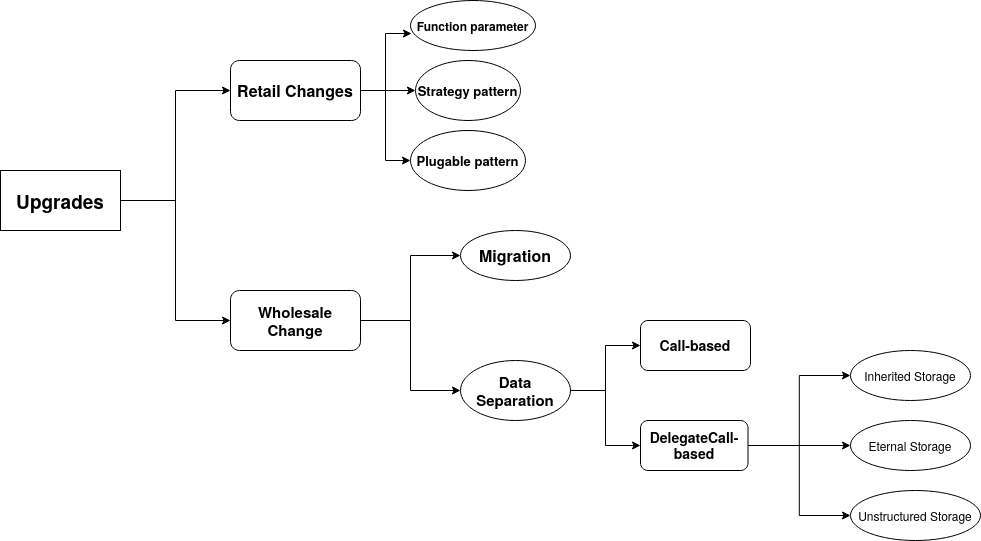
\includegraphics[width=0.9\textwidth]{figures/Chart.png}
  \caption{Classification}
 \end{figure}

 \section{Evaluation of different methods}
%  % compare them using: 
% • Frequency
% • Decentralization
% • Foreknowledge of changes
% • Wholesale changes
% • Gas efficiency
% • Efficiency: gas for those uninformed about upgrades
% • Efficiency: gas for those informed about upgrades

 % talk about vulnerabilities of each here
 \section{Upgrading process}


 \subsection{decision maker(s)}
 There is a debate on who is responsible for upgrading a Dapp. Different systems can choose one of these schemes to upgrade their Dapp depending on the complexity of the system, frequency of the changes needed for the system and how fast does the system need to upgrade in the incidents.

 \subsubsection{Externally owned Address}
The easiest and the fastest way to upgrade a system is through a single address which is the owner of smart contract. This is the most centralized solution we have for upgrading a system. The main problem with this issue is the security of the system because it only depends on a single private key hold by the owner. In case of malicious party or if an attacker find the owner's private or if the owner lose the key the entire system is on the risk.

First Dapps on the ethereum blockchain used this method for the upgrade but it is not used these days because it is far from the idea of \textit{Decentralization}. 

 \subsubsection{Multi-Sig}
 A \textit{m out of n} Multi-sig wallet is a smart contract that can manage a transactions only if m number out of a specified n EOAs agree and sign the transaction. We can use address of a Multi-sig wallet as the owner of the system. In case of a upgrade or responding to an incident m number of the governors can permit to upgrade the system.

 This is a better answer to the decision making of the upgrade compare to using an EOA in case of centrality while keeping the speed of an upgrade process. However, it is not decentralized. One way to reduce the level of centralization is to use different trusted teams who are stakeholders of the system in the multi-sig wallet. 


\subsubsection{Governance Voting}
The most decentralized way to decide on a system change is to do it using decentralized voting. This can be done by distributing governance voting tokens to the community and then they can vote on a change proposal by staking their voting token. 

There are some critique to this method. Governance by voting has an inherit time delay to the upgrading process. This raises a problem when the system needs an instant upgrade (\eg responding to an incident). This means we need another mechanism to quickly fix bugs and upgrade the system on the event of incidents in conjunction with the voting process (\eg Global shutdown in MakerDAO).

It is also not cost-efficient for the voters because all token holders must send a transaction and needs to pay network fee.

The other problem with this method is fair distribution of the tokens. If the governance token does not distribute fairly and the majority of tokens granted to the limited number of users, then it is very similar to the multi-sig method which is more costly and complex. Because, whales of the governance token can vote to any desired change of the system similar to the multi-sig.
 

\subsection{Mitigating risks}
There are critical setups on the systems to mitigate the possible risks on the upgrading process. We mention some of them here with risk associated with them.

\subsubsection{Timelocks}
In some project, there is a time window between every changes that approved on the system and when they affect the system. This gives opportunity to the users who are not satisfied with the upcoming upgrades to move their funds out of the system. However this is not proper in case of fixing a bug, because we need to patch the problem quickly.

\subsubsection{Thereshold}
In multi-sig and governance upgrade methods we need a threshold on votes to decide whether a change is approved or not. This threshold should be big enough to be confident that upgrading event represents the majority of opinions. On the other hand, the threshold shouldn't be that big because a big threshold will delay a system change. The system designer should consider that a portion of voters (signers in multi-sig or governance token holders in voting method) may not be available in the event of the upgrade and having a big threshold may result in halting the change proposal for a long period of time. In fact threshold has a trade-off between security/decentralization and speed of the upgrade process.

\subsubsection{Pausable}
In pauseable smart contracts, the decision makers (usually a multi-sig wallet) can freeze some or all operations of the system. Pausing a smart contract helps in some specific situations:

\begin{enumerate}
  \item Time to react to a bug or hack: usually it takes time to analyze and find the reason of a hack and patch the bug. In this time period the core developer team needs to pause the system to stop attacker from draining all the fund.
  \item Halting system in the upgrade process: For instance, in an ERC20 token contract upgrade we need to pause the system to stop users from transferring tokens during the upgrade. 
  \item Inactivating the previous version of the logic contracts: After an upgrade we need to have a plan to stop users from using the previous logic contracts. One way to do so is to make the logic contracts pauseable and pause them after the upgrade. 
\end{enumerate}

\subsubsection{Escape Hatches}
A escape hatch is a mechanism that lets the users to move their fund out of the system in the pausing events. For instance, in MakerDAO we have an emergency shutdown mechanism that pauses the system in the black swan events. But, users have the ability to extract their funds out of the system while the system is paused.
\subsubsection{Front-Runnign}
Upgrading a smart contract can be done by sending a transaction into the system. If the upgrade is a response to a unknown bug, then the upgrade process will hint attackers who is listening to the mempool to find the bug and hack the smart contract just before the upgrade. So there should be some mechanisms to mitigate front-running attacks. One solution to this issue is to use commit-reveal schemes. The team first sends a commitment of the upgrade (hash of the upgrade) to the system and after the timelock they can push and apply the original code which cannot be front run. 
%Commit reveal



% upgrading in dark: https://forum.makerdao.com/t/mip15-dark-spell-mechanism/2578


 \section{Measurement study}
% Level of intervention of each Dapp (pauseable etc.)
% History of upgrades --> How many times a Dapp upgraded before (using events etc...)

% \section{Concluding Remarks}


% \subsection{Registry pattern}
% Registry contracts are probably the simplest approach to upgradeability. Registry pattern consist of two main contracts: registry and logic contract. Registry contract holds the addresses of logic contracts and whenever it receives a transaction it will pass it to the related logic contract. 
% If the development team decide to upgrade the smart contract, they can deploy another smart contract and then just change the pointer of the registry smart contact to the new smart contract.

% The main disadvantage of this approach is that in upgrading event, there should be a manual or automated migration plan to transfer data from the old contract into the new upgrade smart contract.
% Another drawback of this pattern is that it also introduces additional complexity for external clients who would also need to call into the registry before interacting with the system


%Idea: see how frequent each project uses its upgradeability feature to upgrade the contract and why?

%In proxy storage layout you should take care that: 
% 1. never remove variable
% 2. never change var type
% 3. never change inheritance order


%Implementation of Eternal storage in call based upgrades: https://medium.com/cardstack/upgradable-contracts-in-solidity-d5af87f0f913
% Good classificaton: https://medium.com/1milliondevs/solidity-storage-layout-for-proxy-contracts-and-diamonds-c4f009b6903
% New storage type *Dimond Storage*: https://medium.com/1milliondevs/new-storage-layout-for-proxy-contracts-and-diamonds-98d01d0eadb
%https://medium.com/1milliondevs/new-storage-layout-for-proxy-contracts-and-diamonds-98d01d0eadb
% Upgradability checklist: https://blog.trailofbits.com/2020/06/12/upgradeable-contracts-made-safer-with-crytic/



%ToDo: Write about OpenZeppling upgrade bug : https://blog.trailofbits.com/2018/09/05/contract-upgrade-anti-patterns/
%ToDo: Gas cost comparison between different implementation (using different number and types of the storage variables)